\section{ XSLT}

\begin{frame}[fragile]{CH7 XSLT}
\begin{figure}
    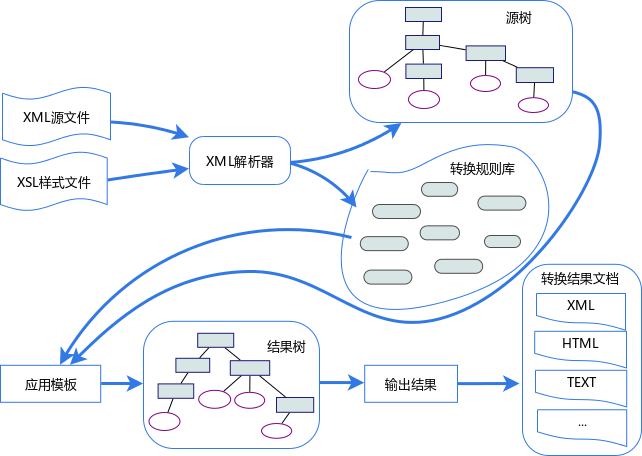
\includegraphics[width=0.9\textwidth]{figure/xslt.png}
\end{figure}
\end{frame}

\begin{frame}[fragile]{本章学习目标}
\begin{easylist} \easyitem
& 了解XSLT的发展历史、XSLT与XSL的关系
& 掌握XSLT的转换处理过程
& 掌握XSLT的基本语法
& 能够使用SAXON进行XSLT测试
\end{easylist}
\end{frame}

\begin{frame}[fragile]{目录}
\begin{easylist} \easyitem
& XSLT概述
& 如何测试XSLT
& XSLT快速入门
& XSLT的输出格式控制
& XSLT的逻辑处理元素
& XSLT的模式
& XSLT的命名模板
& XSLT的函数
& XSLT 2.0
\end{easylist}
\end{frame}


\subsection{7.1 概述}

\begin{frame}[fragile]{7.1 概述}
\begin{easylist} \easyitem
& XSLT与XSL
& XSLT的作用
& XSLT的工作流程
& XSLT的应用模式
& XSLT与CSS的区别
\end{easylist}
\end{frame}


\subsubsection{7.1.1 XSLT与XSL}
\begin{frame}[fragile, allowframebreaks]{7.1.1 XSLT与XSL}
\begin{easylist} \easyitem
& XSLT
&& 可扩展样式语言转换(Extensible Stylesheet Language Transformations)
&& 可扩展样式语言XSL(Extensible Stylesheet Language)的一个组成部分
& XSL
&& 定义XML文档的格式化和呈现方式,以方便在屏幕、纸张等媒介上显示或通过语音输出
&& 包含两个相对独立的阶段:
&&& 结构转换阶段:实现XML文档元素的选择、分组、重新排列
&&& 格式化处理阶段,实现具体的呈现功能

&& XSL又被拆分为两部分:
&&& XSLT用于定义转换
&&& 剩余的部分——仍称为XSL,也有人称之为XSL-FO(XSL Formatting)

&& XSL目前包含三个组成部分
&&& XSL转换XSLT:描述如何把一个XML文档转换为另外一个文本格式的文档,如XML文档或HTML文档
&&& XML路径语言XPath:在XSLT之中实现存取或引用XML文档特定部分的表达式语言
&&& XSL格式化对象(XSL Formatting Objects, XSL-FO):定义XML文档的格式化显示方式
\end{easylist}
\end{frame}


\subsubsection{7.1.2 XSLT的作用}
\begin{frame}[fragile]{7.1.2 XSLT的作用}
\begin{easylist} \easyitem
& 把一个XML文档转换为另一个类型的文档,可以在输出文档里增删元素和属性,可以对源文档的元素进行重新排列,并有选择的组织显示
& 常见的三种转换
\begin{figure}
    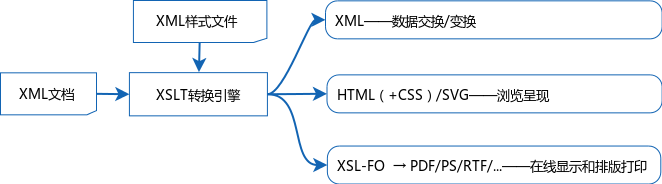
\includegraphics[width=0.85\textwidth]{figure/xslt-transform.png}
\end{figure}
\end{easylist}
\end{frame}


\begin{frame}[fragile]{把一个版本的XML转换为另一个版本}
\begin{lstlisting}[tabsize=8, basicstyle=\small\tt, language=XML]
<v1:order xmlns:v1="http://www.test.com/v1"> 
    <product name="打印纸" price="30" quantity="5"/>
</v1:order>
\end{lstlisting}

\begin{lstlisting}[tabsize=8, basicstyle=\small\tt, language=XML]
<v2:order xmlns:v2="http://www.test.com/v2">
    <product quantity="5">
        <name>打印纸</name>
        <price>30</price>
    </product>
</v2:order>
\end{lstlisting}
\end{frame}


\begin{frame}[fragile]{把XML转换为HTML}
\begin{lstlisting}[tabsize=8, basicstyle=\small\tt, language=HTML]
<html>
    <head><title>Order Details</title></head>
    <body>
        <p>名称:打印纸</p>
        <p>单价:30元;数量:5 </p>
    </body>
</html>
\end{lstlisting}
\end{frame}


\subsubsection{7.1.3 XSLT的工作流程}
\begin{frame}[fragile]{7.1.3 XSLT的工作流程}
\begin{easylist} \easyitem
\begin{figure}
    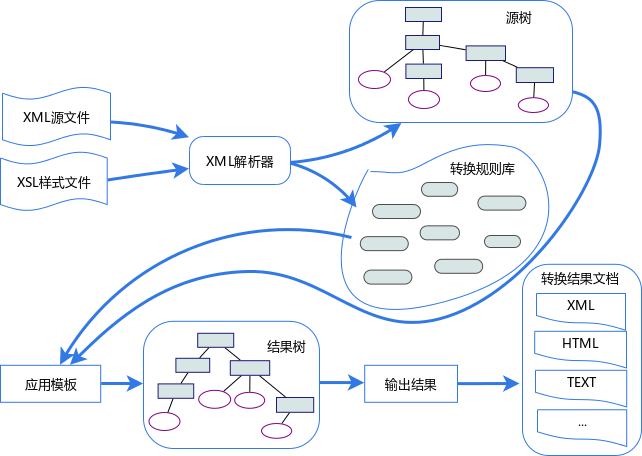
\includegraphics[width=0.75\textwidth]{figure/xslt.png}
\end{figure}
\end{easylist}
\end{frame}


\subsubsection{7.1.4 XSLT的应用模式}
\begin{frame}[fragile]{7.1.4 XSLT的应用模式}
\begin{easylist} \easyitem
& 服务器端应用模式
&& 转换是在服务器端完成
& 客户端应用模式
&& 转换由客户端的浏览器完成
& 独立模式
&& 转换由独立程序完成,如Saxon
\end{easylist}
\end{frame}


\subsubsection{7.1.5 XSLT与CSS的区别}
\begin{frame}[fragile]{7.1.5 XSLT与CSS的区别}
\begin{easylist} \easyitem
& 转换动作不同
&& XSLT采用转换方式,把XML文档由一种格式转换为另一种格式;CSS无转换动作,只是针对XML元素设定显示样式。
& 互动性不同
&& CSS可以实现闪烁等动态效果,XSLT转换本身则没有这方面的功能。
& 语法不同
&& XSL样式文件为标准的XML文件,而CSS的语法自成一格
\end{easylist}
\end{frame}



\subsection{7.2 如何测试XSLT}

\begin{frame}[fragile]{7.2 如何测试XSLT}
\begin{easylist} \easyitem
& 浏览器
& XML工具
& 独立的XSLT处理器
\end{easylist}
\end{frame}


\subsubsection{7.2.1 通过浏览器测试XSLT}
\begin{frame}[fragile]{7.2.1 通过浏览器测试XSLT}
\begin{easylist} \easyitem
& 在XML文档中通过<?xml-stylesheet?>处理指令进行样式的关联
& 通过浏览器打开XML文档查看转换效果
& 看不到转换结果的源代码
\end{easylist}
\end{frame}


\subsubsection{7.2.2 通过XML专业工具测试}
\begin{frame}[fragile]{7.2.2 通过XML专业工具测试}
\begin{figure}
    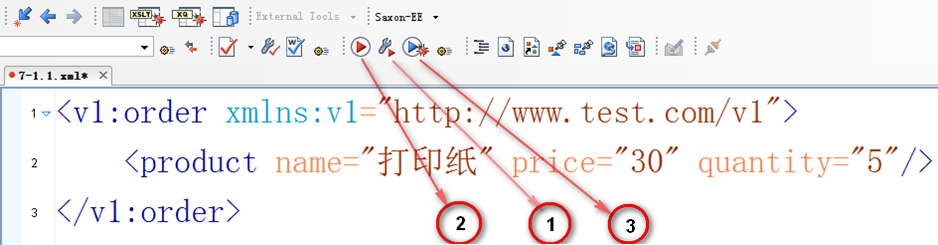
\includegraphics[width=0.85\textwidth]{figure/xslt-oxygen-test.png}
\end{figure}
\end{frame}


\subsubsection{7.2.3 通过XSLT处理器测试}
\begin{frame}[fragile]{7.2.2 通过XSLT处理器测试}
\begin{easylist} \easyitem
& Saxon
&& 安装Java
&& 下载并配置Saxon
&& 指定参数实现样式转换
&&& 语法:
&&&& java -jar saxon9he.jar -s:source -xsl:stylesheet -o:output
&&& 例子:
&&&& java -jar saxon9he.jar -s:7-1.1.xml -xsl:7-1.2.xsl -o:7-1.out.xml
\end{easylist}
\end{frame}


\subsection{7.3 XSLT快速入门}

\begin{frame}[fragile, allowframebreaks]{7.3 XSLT快速入门}
\begin{lstlisting}[tabsize=8, basicstyle=\small\tt, language=XML, caption="7-2.xml"]
<?xml version="1.0"?>
<books>
    <provider>Summer</ provider>
    <book isbn="978-7-115-21703-5">
        <title>Python高级编程</title>
        <price>45.00</price>
        <authors>
            <author>Tarek Ziade</author>
            <author type="translator">姚军</author>
            <author type="translator">夏海伦</author>
            <author type="translator">王秀丽</author>
        </authors>
        <press>人民邮电出版社</press>
        <pages>306</pages>
        <description>介绍了Python语言的最佳实践和敏捷开发方法…</description>
        <cover>book-python.jpg</cover>
    </book>
    <book isbn="978-7-115-28282-8">
        <title>数学之美</title>
        <price>45.00</price>
        <authors>
            <author>吴军</author>
        </authors>
        <press>人民邮电出版社</press>
        <pages>304</pages>
        <description>读了“数学之美”,才发现大学时学的数学知识…</description>
        <cover>book-math.jpg</cover>
    </book>
    <book isbn="978-7-5641-1139-7">
        <title>集体智慧编程(影印版)</title>
        <price>58.00</price>
        <authors>
            <author>Toby Segaran</author>
        </authors>
        <press>东南大学出版社</press>
        <pages>334</pages>
        <description>Toby的书非常成功地将复杂的机器学习算法问题…</description>
        <cover>book-collective.jpg</cover>
    </book>
</books>
\end{lstlisting}

\begin{lstlisting}[tabsize=8, basicstyle=\small\tt, language=XML, caption="7-2.xsl"]
<?xml version="1.0" encoding="UTF-8"?>
<xsl:stylesheet xmlns:xsl="http://www.w3.org/1999/XSL/Transform" version="2.0">
    <xsl:template match="/">
    <html>
        <head><title>图书列表</title></head>
        <body>
            <xsl:apply-templates/>
        </body>
    </html>
    </xsl:template>
    <xsl:template match="books">
        <table>
            <xsl:apply-templates select="book"/>
        </table>
    </xsl:template>
    <xsl:template match="book">
        <tr>
            <td><xsl:value-of select="title"/></td>
        </tr>
    </xsl:template>
</xsl:stylesheet>
\end{lstlisting}

\begin{shaded}
java -jar saxon9he.jar -s:7-2.xml -xsl:7-2.xsl -o:7-2.out.html
\end{shaded}


\begin{lstlisting}[tabsize=8, basicstyle=\small\tt, language=HTML, caption="7-2.out.html"]
<html>
    <head>
        <meta http-equiv="Content-Type" content="text/html; charset=UTF-8">
        <title>图书列表</title>
    </head>
    <body>
        <table>
            <tr><td>Python高级编程</td></tr>
            <tr><td>数学之美</td></tr>
            <tr><td>集体智慧编程(影印版)</td></tr>
        </table>
    </body>
</html>
\end{lstlisting}

\begin{shaded}
利用<?xml-stylesheet?>处理指令在“7-2.xml”中建立与“7-2.xsl”的关联,通过浏览器查看结果
\end{shaded}

\begin{figure}
    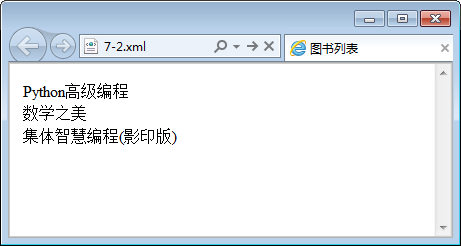
\includegraphics[width=0.75\textwidth]{figure/xslt-7-2.out.png}
\end{figure}
\end{frame}


\subsubsection{7.3.1 stylesheet元素}
\begin{frame}[fragile]{7.3.1 stylesheet元素}
\begin{lstlisting}[tabsize=8, basicstyle=\small\tt, language=XML, numbers=none]
<xsl:stylesheet xmlns:xsl="http://www.w3.org/1999/XSL/Transform" version="2.0">
\end{lstlisting}
\end{frame}


\subsubsection{7.3.2 template元素}
\begin{frame}[fragile]{7.3.2 template元素}
\begin{lstlisting}[tabsize=8, basicstyle=\small\tt, language=XML, numbers=none]
<xsl:template match="要匹配的模式串"
            name="名称"
            priority="代表优先级的数字">
    <!—模板的具体内容 -->
</xsl:template>
\end{lstlisting}
\end{frame}


\subsubsection{7.3.3 apply-templates元素}
\begin{frame}[fragile]{7.3.3 apply-templates元素}
\begin{lstlisting}[tabsize=8, basicstyle=\small\tt, language=XML, numbers=none]
<xsl:template match="/books">
    <xsl:apply-templates select="book "/>
</xsl:template>
\end{lstlisting}

\begin{lstlisting}[tabsize=8, basicstyle=\small\tt, language=XML, numbers=none]
<xsl:template match="/books">
    <xsl:apply-templates/>
</xsl:template>
\end{lstlisting}
\end{frame}


\subsubsection{7.3.4 value-of元素}
\begin{frame}[fragile]{7.3.4 value-of元素}
\begin{easylist} \easyitem
& 根据select属性值从源树中读取信息
& xsl:value-of在XSLT的1.0和2.0版本中转换行为不一致
\begin{lstlisting}[tabsize=8, basicstyle=\small\tt, language=XML, numbers=none]
<xsl:value-of select="author"/>
\end{lstlisting}
&& 在1.0中,仅选取第一个结点的值,结果为:Tarek Ziade
&& 在2.0中,顺序输出所有的结点,默认通过空格分隔:Tarek Ziade 姚军 夏海伦 王秀丽
&& 可更换分隔符,如下:
\begin{lstlisting}[tabsize=8, basicstyle=\small\tt, language=XML, numbers=none]
<xsl:value-of select="author" separator=","/>
\end{lstlisting}
&& 此时结果为:Tarek Ziade,姚军,夏海伦,王秀丽
\end{easylist}
\end{frame}


\subsubsection{7.3.5 attribute元素}
\begin{frame}[fragile]{7.3.5 attribute元素}
\begin{easylist} \easyitem
& 生成属性信息,例如:
\begin{lstlisting}[tabsize=8, basicstyle=\small\tt, language=XML, numbers=none]
<img>
    <xsl:attribute name="src"><xsl:value-of select="cover"/></xsl:attribute>
    <xsl:attribute name="width">80</xsl:attribute>
    <xsl:attribute name="height">100</xsl:attribute>
</img>
\end{lstlisting}
& 结果:
\begin{lstlisting}[tabsize=8, basicstyle=\small\tt, language=HTML, numbers=none]
<img src="book-python.jpg" width="80" height="100"/>
\end{lstlisting}
\end{easylist}
\end{frame}



\subsection{7.4 XSLT的输出格式控制}
\begin{frame}[fragile]{7.4 XSLT的输出格式控制}
\begin{easylist} \easyitem
& 用于指定转换生成的文档格式:
&& XML、HTML、XHTML或纯文本格式
& 例如:声明转换结果的文本为纯文本格式
\begin{lstlisting}[tabsize=8, basicstyle=\small\tt, language=XML, numbers=none]
<xsl:output method="text"/>
\end{lstlisting}
& method的取值:
&& text、xml、xhtml或html
& XSLT 1.0不支持该指令
\end{easylist}
\end{frame}


\subsection{7.5 XSLT的逻辑处理元素}
\begin{frame}[fragile]{7.5 XSLT的逻辑处理元素}
\begin{easylist} \easyitem
& 条件处理元素
&& if
&& choose
& 循环:for-each
& 排序:sort
\end{easylist}
\end{frame}


\subsubsection{7.5.1 条件处理元素}
\begin{frame}[fragile, allowframebreaks]{if元素}
\begin{lstlisting}[tabsize=8, basicstyle=\small\tt, language=XML, caption=样式文档]
<xsl:stylesheet xmlns:xsl="http://www.w3.org/1999/XSL/Transform" version="2.0">
    <xsl:template match="/">
        <html><body>
            <xsl:apply-templates select="books/book"/>
        </body></html>
    </xsl:template>
    <xsl:template match="book">
        <xsl:if test="price &lt; 50">
            <p><xsl:value-of select="title"/></p>
        </xsl:if>
    </xsl:template>
</xsl:stylesheet>
\end{lstlisting}

\begin{lstlisting}[tabsize=8, basicstyle=\small\tt, language=HTML, caption=转换结果]
<html>
    <body>
        <p>Python高级编程</p>
        <p>数学之美</p>
    </body>
</html>
\end{lstlisting}
\end{frame}


\begin{frame}[fragile, allowframebreaks]{choose元素}
\begin{lstlisting}[tabsize=8, basicstyle=\small\tt, language=XML, caption=样式文档]
<xsl:stylesheet xmlns:xsl="http://www.w3.org/1999/XSL/Transform" version="2.0">
    <xsl:template match="/">
        <html><body>
            <xsl:apply-templates select="books/book"/>
        </body></html>
    </xsl:template>
    <xsl:template match="book">
        <xsl:choose>
            <xsl:when test="price &lt; 50"><p><xsl:value-of select="title"/></p></xsl:when>
            <xsl:when test="price &lt; 100"><p>* <xsl:value-of select="title"/></p></xsl:when>
            <xsl:otherwise><p># <xsl:value-of select="title"/></p></xsl:otherwise>
        </xsl:choose>
    </xsl:template>
</xsl:stylesheet>
\end{lstlisting}

\begin{lstlisting}[tabsize=8, basicstyle=\small\tt, language=HTML, caption=转换结果]
<html>
    <body>
        <p>Python高级编程</p>
        <p>数学之美</p>
        <p>*集体智慧编程(影印版)</p>
    </body>
</html>
\end{lstlisting}
\end{frame}


\subsubsection{7.5.2 循环元素for-each}
\begin{frame}[fragile, allowframebreaks]{for-each元素}
\begin{lstlisting}[tabsize=8, basicstyle=\small\tt, language=XML, caption=样式文档]
<xsl:stylesheet xmlns:xsl="http://www.w3.org/1999/XSL/Transform" version="2.0">
    <xsl:template match="/">
        <html><body>
            <xsl:apply-templates select="books"/>
        </body></html>
    </xsl:template>
    <xsl:template match="books">
        <xsl:for-each select="book">
            <p><xsl:value-of select="title"/></p>
        </xsl:for-each>
    </xsl:template>
</xsl:stylesheet>
\end{lstlisting}

\begin{lstlisting}[tabsize=8, basicstyle=\small\tt, language=HTML, caption=转换结果]
<html>
    <body>
        <p>Python高级编程</p>
        <p>数学之美</p>
        <p>集体智慧编程(影印版)</p>
    </body>
</html>
\end{lstlisting}
\end{frame}


\subsubsection{7.5.3 排序元素sort}
\begin{frame}[fragile, allowframebreaks]{sort元素}
\begin{lstlisting}[tabsize=8, basicstyle=\small\tt, language=XML, caption=样式文档]
<xsl:stylesheet xmlns:xsl="http://www.w3.org/1999/XSL/Transform" version="2.0">
    <xsl:template match="/">
        <html><body>
            <xsl:apply-templates select="books"/>
        </body></html>
    </xsl:template>
    <xsl:template match="books">
        <xsl:for-each select="book">
            <xsl:sort select="price" order="descending"/>
            <p><xsl:value-of select="title"/></p>
        </xsl:for-each>
    </xsl:template>
</xsl:stylesheet>
\end{lstlisting}

\begin{lstlisting}[tabsize=8, basicstyle=\small\tt, language=HTML, caption=转换结果]
<html>
    <body>
        <p>集体智慧编程(影印版)</p>
        <p>Python高级编程</p>
        <p>数学之美</p>
    </body>
</html>
\end{lstlisting}
\end{frame}



\subsection{7.6 XSLT的模式-mode}
\begin{frame}[fragile, allowframebreaks]{7.6 XSLT的模式-mode}
\begin{lstlisting}[tabsize=8, basicstyle=\small\tt, language=XML, caption=样式文档]
<xsl:stylesheet xmlns:xsl="http://www.w3.org/1999/XSL/Transform" version="2.0">
    <xsl:template match="/">
        <html><body>
            <h2>按照价格降序排列的图书名称</h2>
            <xsl:apply-templates select="books" mode="simple"/>
            <h2>图书详细列表</h2>
            <xsl:apply-templates select="books" mode="detail"/>
        </body></html>
    </xsl:template>
    <xsl:template match="books" mode="simple">
        <ul>
            <xsl:for-each select="book">
                <xsl:sort select="price" order="descending"/>
                <li><xsl:value-of select="title"/></li>
            </xsl:for-each>
        </ul>
    </xsl:template>
    
    <xsl:template match="books" mode="detail">
        <table>
            <tr>
                <td>ISBN</td><td>标题</td><td>作者</td><td>出版社</td><td>价格</td>
            </tr>
            <xsl:for-each select="book">
                <xsl:sort select="pages" order="ascending"/>
                <tr>
                    <td><xsl:value-of select="@isbn"/></td>
                    <td><xsl:value-of select="title"/></td>
                    <td><xsl:value-of select="authors"/></td>
                    <td><xsl:value-of select="press"/></td>
                    <td><xsl:value-of select="price"/></td>
                    <td><img><xsl:attribute name="src" select="cover"/></img></td>
                </tr>
            </xsl:for-each>
        </table>
    </xsl:template>
</xsl:stylesheet>
\end{lstlisting}

\begin{lstlisting}[tabsize=8, basicstyle=\small\tt, language=HTML, caption=转换结果]
<html>
    <body>
        <h2>按照价格降序排列的图书名称</h2>
        <ul>
            <li>集体智慧编程(影印版)</li>
            <li>Python高级编程</li>
            <li>数学之美</li>
        </ul>
        <h2>图书详细列表</h2>
        <table>
            <tr>
                <td>ISBN</td><td>标题</td><td>作者</td><td>出版社</td><td>价格</td>
            </tr>
            <tr>
                <td>978-7-115-28282-8</td>
                <td>数学之美</td>
                <td>吴军</td>
                <td>人民邮电出版社</td>
                <td>45.00</td>
                <td><img src="book-math.jpg"></td>
            </tr>
            <tr>
                <td>978-7-115-21703-5</td>
                <td>Python高级编程</td>
                <td>Tarek Ziade 姚军 夏海伦 王秀丽</td>
                <td>人民邮电出版社</td>
                <td>45.00</td>
                <td><img src="book-python.jpg"></td>
            </tr>
            <tr>
                <td>978-7-5641-1139-7</td>
                <td>集体智慧编程(影印版)</td>
                <td>Toby Segaran</td>
                <td>东南大学出版社</td>
                <td>58.00</td>
                <td><img src="book-collective.jpg"></td>
            </tr>
        </table>
    </body>
</html>
\end{lstlisting}
\end{frame}



\subsection{7.7 XSLT的命名模版}
\begin{frame}[fragile, allowframebreaks]{7.7 XSLT的命名模版}
\begin{easylist} \easyitem
& 模版定义语法:
\begin{lstlisting}[tabsize=8, basicstyle=\small\tt, language=XML, numbers=none]
<xsl:template name="模板名称">
    <!—模板的具体内容 -->
</xsl:template>
\end{lstlisting}
& 定义好的模板通过xsl:call-template指令进行调用
& 示例:
\end{easylist}
\begin{lstlisting}[tabsize=8, basicstyle=\small\tt, language=XML, caption=样式文档]
<xsl:stylesheet xmlns:xsl="http://www.w3.org/1999/XSL/Transform" version="2.0">
    <xsl:template match="/">
        <html><body>
            <h2>图书提供者信息</h2>
            <xsl:call-template name="providerTemplate"/>
            <h2>按照价格降序排列的图书名称</h2>
            <xsl:apply-templates select="books" mode="simple"/>
            <h2>图书详细列表</h2>
            <xsl:apply-templates select="books" mode="detail"/>
        </body></html>
    </xsl:template>
    
    <xsl:template name="providerTemplate">
        <p>本图书列表由:
        <strong><xsl:value-of select="/books/provider"/></strong>提供.
        </p>
    </xsl:template>
    
    <xsl:template match="books" mode="simple">
        <!-- 省略,同7-7.xsl对应内容… -->
    </xsl:template>
    
    <xsl:template match="books" mode="detail">
        <!-- 省略,同7-7.xsl对应内容… -->
    </xsl:template>
</xsl:stylesheet>
\end{lstlisting}

\begin{lstlisting}[tabsize=8, basicstyle=\small\tt, language=HTML, caption=转换结果]
<html>
    <body>
        <h2>图书提供者信息</h2>
        <p>本图书列表由:<strong>Summer</strong>提供. </p>
        <h2>按照价格降序排列的图书名称</h2>
        <!-- 以下内容与7-7.out.html相同,此处省略… -->
    </body>
</html>
\end{lstlisting}
\end{frame}



\subsection{7.8 XSLT的函数}
\begin{frame}[fragile, allowframebreaks]{7.8 XSLT的函数}
\begin{easylist} \easyitem
& 可以直接使用XPath的函数
& XSLT本身的函数
&& document()
&& key()
&& format-number()
&& generate-id()
& 示例:
\end{easylist}
\begin{lstlisting}[tabsize=8, basicstyle=\small\tt, language=XML, caption=样式文档]
<xsl:stylesheet xmlns:xsl="http://www.w3.org/1999/XSL/Transform" version="2.0">
    <xsl:template match="/">
        <html><body>
            <h2>图书平均价格信息</h2>
            <xsl:call-template name="priceTemplate"/>
        </body></html>
    </xsl:template>
    <xsl:template name="priceTemplate">
    平均价格:
    <xsl:value-of select="format-number(sum(/books/book/price) div count(/books/book/price), '0')"/>
    </xsl:template>
</xsl:stylesheet>
\end{lstlisting}

\begin{lstlisting}[tabsize=8, basicstyle=\small\tt, language=HTML, caption=转换结果]
<html>
    <body>
        <h2>图书平均价格信息</h2>
        平均价格:49
    </body>
</html>
\end{lstlisting}
\end{frame}


\subsection{7.9 XSLT 2.0新特性}
\begin{frame}[fragile]{7.9 XSLT 2.0新特性}
\begin{easylist} \easyitem
& 新增数据模型
& 支持Schema数据类型
& 新增元素和函数
& 支持非XML输入源
& 改进了字符处理
& 支持多文件输出
\end{easylist}
\end{frame}



\begin{frame}
\begin{center}
    \Huge END
\end{center}
\begin{figure}
    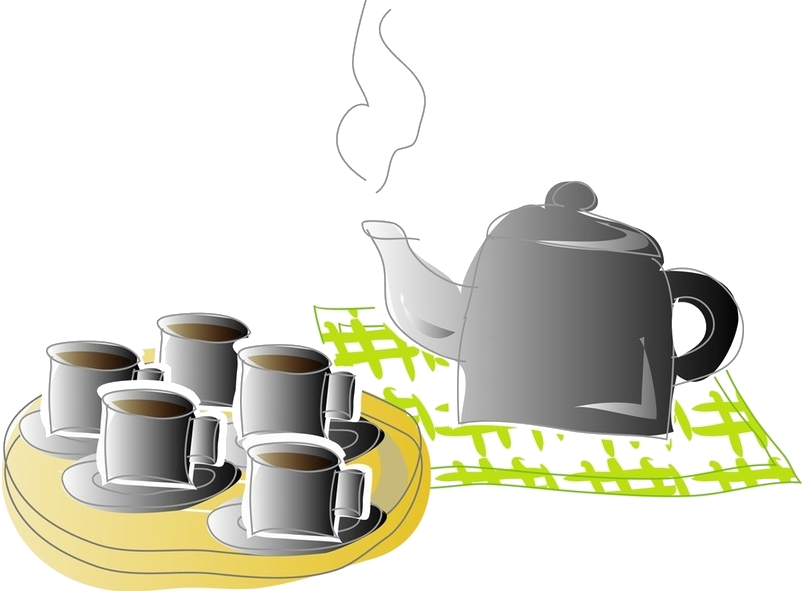
\includegraphics[width=0.75\textwidth]{figure/relax.png}
\end{figure}
\end{frame}
